\section{PIA}
La PIA è un dispositivo di comunicazione parallela ad 8 bit. Tale architettura è un dispositivo hardware che si posiziona tra la periferica e il processore stesso. Essa è costituita architetturalmente da due tipologie diverse di porto, il porto A ed il porto B.[\ref{img:PIA}]
Tali porti hanno dei registri che sono direzionali, quindi possono assumere una sola funzione (tra entrata ed uscita), in base alla loro specifica impostazione e configurazione.
Prima di parlare di più porti ci concentriamo sulle comunicazioni a singolo porto; in generale le comunicazioni che avvengono tra due interfacce della PIA sono configurabili tramite i bit di configurazione del chipset. Nel nostro caso, la comunicazione che maggiormente utilizzeremo è quella dotata di handshacking, per cui si avrà una configuraizone ed un collegamento simile all'immagine [\ref{img:PIA-CON}]. Entrando nei dettagli del processo, bisognerà fare particolare attenzione ai seguenti registri:
\begin{itemize}
    \item \textbf{CA1,CB1}: Sono registri che possono assumere solo direzione di ingresso e solitamente vengono usati come "lettori" di segnali SYN o segnali ACK da parte dell'altro dispositivo. CIao a tutti
    \item \textbf{CA2,CB2}: Sono i registri che possono essere configurati(sia di ingresso che di uscita), ed in generale, in base al protocollo che si vuole interpretare, vengono settati in una determinata modalità di funzionamento (dipendente dalla tipologia di protocollo che si vuole implementare)
    \item \textbf{Dato}: Il bus dati trasmette parallelamente i dati tra le due periferiche in base al protocollo di handshacking utilizzato
\end{itemize}

\begin{figure}
    \centering
    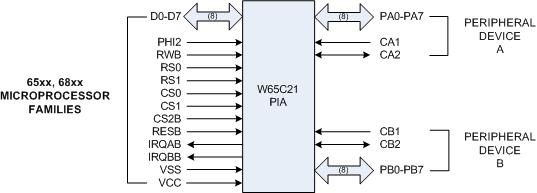
\includegraphics[width=0.45\textwidth]{img/PIA.png}
    \hfill
    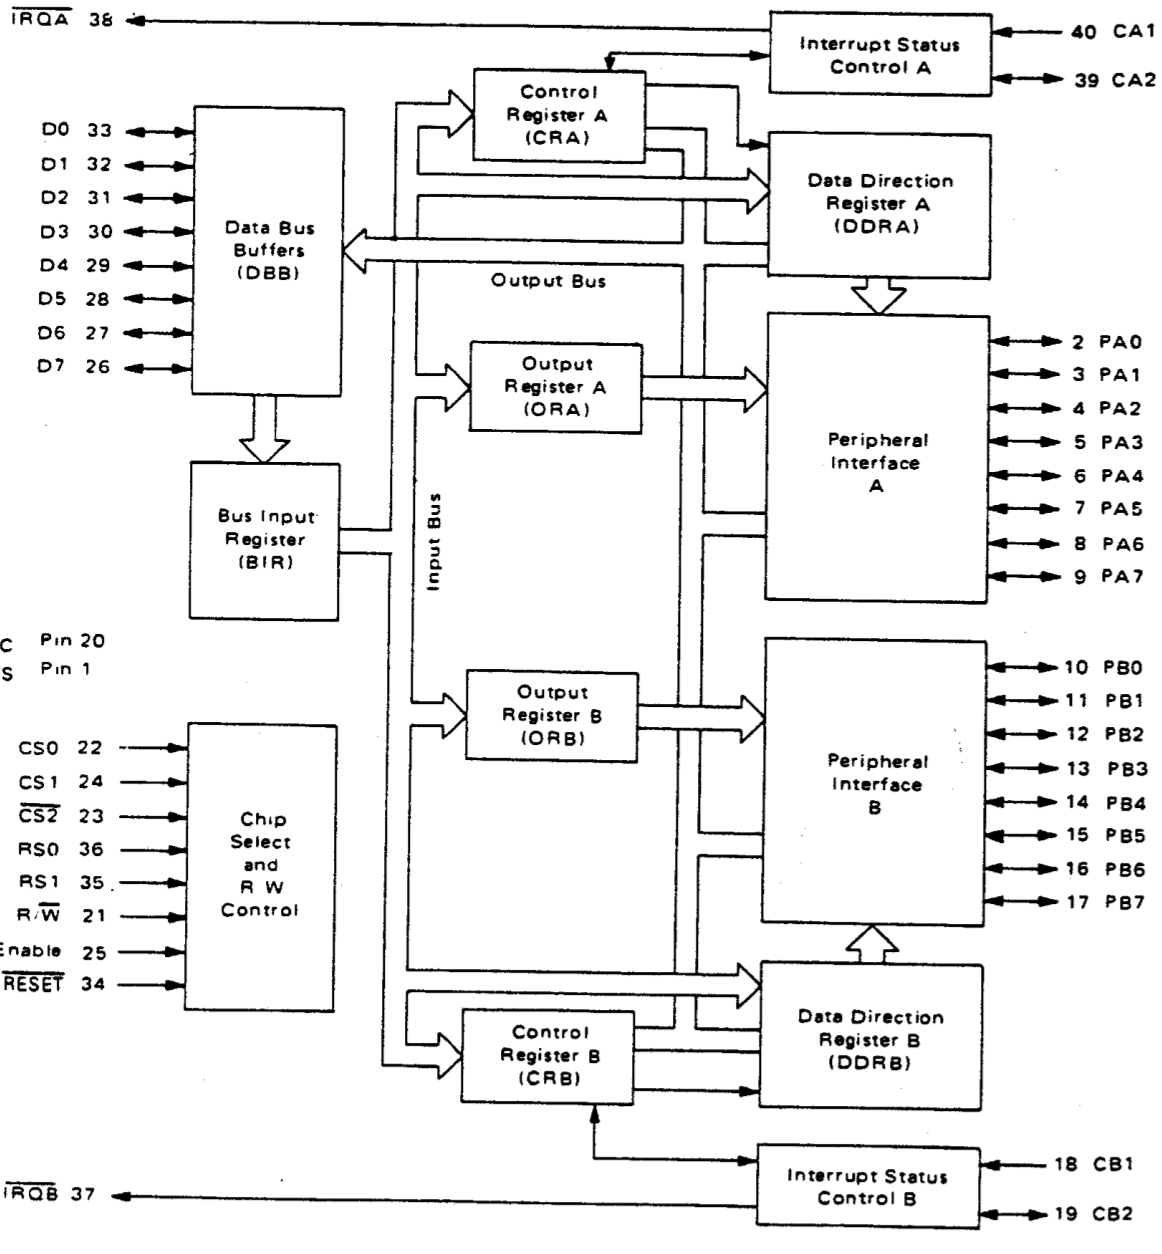
\includegraphics[width=0.45\textwidth]{img/PIA-SCHEME.jpg}
    \caption{Architettura base della PIA}\label{img:PIA}
\end{figure}

\begin{figure}
    \centering
    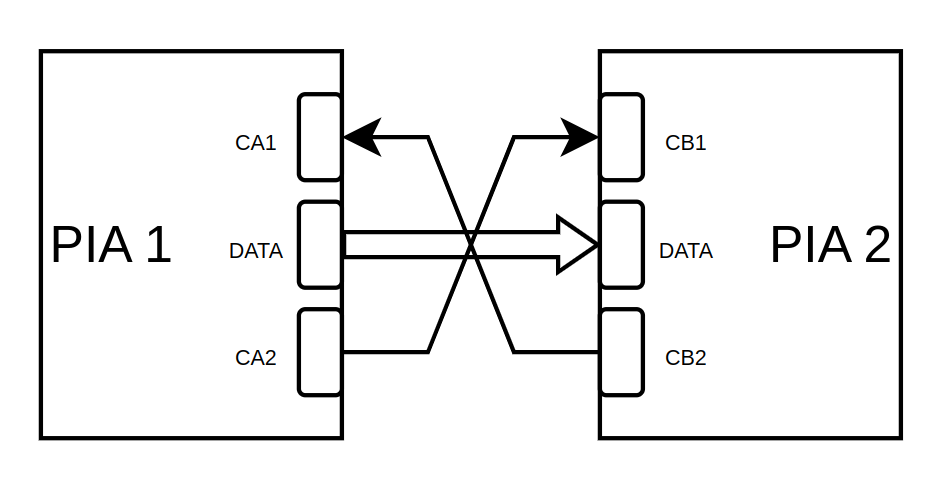
\includegraphics[width=0.65\textwidth]{img/PIA-CON.png}
    \caption{Collegamento tra due dispositivi tramite PIA}\label{img:PIA-CON}
\end{figure}
Per far si che le due architetture possano comunicare è quindi importante definire come si andranno a collegare e quindi la direzione e l'interpretazione che devo andare a dare ai registri. Una possibile architettura di collegamento è quella visibile all'immagine [\ref{img:PIA-CON}].
Una volta definita la tipologia di architettura si va a decidere come queste periferiche dovranno interagire tra loro (definizione del protocollo o modello di programmazione della PIA), per cui si va ad impostare uno specifico registro di configurazione che permetterà di impostare le seguenti opzioni:
\begin{itemize}
    \item \textbf{Interrupt o polling}: A che livello di priorità si andrà ad impostare l'interruzione della PIA
    \item \textbf{Modalità di funzionamento}: se attuo l'hanshacking o altre tipologie di perotocolli
    \item \textbf{Lettura o scrittura}: 

 
\end{itemize}
Una volta definita la struttura del registro di configurazione questo viene settato per impostare la PIA. 
Una volta impostato il modo di funzionamento si va a gestire il tutto. Qundi, se si è scelto un funzionamento tramite interrupt si avrà un certo tipo di comportamento, altrimenti se ne avrà un altro.

Il funzionamento generale della fase di handshacking tra due dispositivi PIA è gestita, per i nostri esempi, in un particolare modo.
Per fare chiarezza andremo a dividere la fase di ricezione dalla fase di trasmissione.
In fase di \textbf{trasmissione} le operazioni che si vanno ad effettuare sonno le seguenti:
\begin{itemize}
    \item \textbf{Inserimento del dato}: Vado a posizionare il dato sui bu dato collegati in maniera diretta con la PIA. Una volta effettuato l'inserimento, la PIA va ad abbassare, in maniera automatica il bit di controllo CA2
    \item \textbf{Attesa dell'ack}: Il sistema aspetta che l'ack si abbassi per capire che il dato è stato inviato correttamente, in questo momento, dato l'abbassamento del segnali in sola lettura su CA1, si alzerà anche il bit di controllo CRA7
    \item \textbf{Lettura fittizzia}: Dato che voglio inviare un nuovo dato, ho bisogno di abbassare il bit CRA7, ma non posso farlo in maniera diretta (configurando un apposito registro di controllo), poichè il bit CRA7 è in sola lettura. Di conseguenza per abbassare tale valore vado ad effettuare una lettura a vuoto (o lettura fittizzia), che mi permette di abbassare il bit e di poter proseguire nelle mie operazioni.
\end{itemize}

Nella fase di ricezione, invece, si ha:
\begin{itemize}
    \item \textbf{Attesa del dato}: Si attende che venga inviato un dato sul porto della PIA, tale attesa può essere effettuata, o tramite Polling andando a controllare in continuazione il valore del bit CRB7 o attivando un interrupt diretta all'arrivo dell'evento sul bit CB1.
    
    \item \textbf{Ricezione del dato}: Una volta compreso che vi è un dato pronto, si effettua una lettura del dato, ed in automatico, la PIA abbasserà il bit CRB7 ed invierà un segnale di ACK, abbassando il valore in CB2

    \item \textbf{Fine}: Nel caso di polling, il sistema continuerà ad aspettare nuovi dati andando a controllare il bit CRB7. Mentre nel caso elle interrupt continuerà il suo normale flusso di esecuzione
\end{itemize}

Andando ad analizzare il codice delle varie operazioni è importante capire la metodologia di funzionamento del sistema, sia per costruire l'architettura in maniera adeguata che per scrivere i driver in maniera corretta.

\subsection{Configurazione della PIA}
La PIA prima di essere utilizzata, richiede una propria configurazione, in parte dipendente dall'architettura e da una parte inerente al driver che si deve implementare.
Per la parte hardware dobbiamo scrivere (almeno per le nostre simulazioni in ASIM), il \textbf{file di configurazione} che definisce tutti gli specifici collegamenti tra i dispositivi con gli specifici significati. Mentre nel caso di configurazione del driver, una volta definita l'architettura su cui si andrà ad eseguire il codice, si vanno ad impostare i registri di controllo e dato, in modo da poter utilizzare il nostro dispositivo (sia con il polling che senza)

\subsubsection{Definizione del file di configurazione}
< chiedere all'assistente o al professore il significato delle varie sigle del file di configurazione >

\subsubsection{Definizione dei registri di controllo e dato}\label{par:cnt-stt}
Il registro di controllo ed il registro di stato vengono definiti all'interno della configurazione. Quindi prima di iniziare a scrivere il driver bisogna osservare per bene il file di configurazione. Più precisamente dobbiamo osservare i seguenti due parametri della nostra PIA:
\begin{itemize}
    \item \textbf{Address 1}: Indirizzo su cui è mappata la PIA
    \item \textbf{Address 2}: Indirizzo del registro di controllo della PIA (dove saranno inserite le configurazioni)
\end{itemize}

Una volta osservati tali parametri si vanno a settare i registri di dato e controllo nel seguente modo:
\begin{lstlisting}
PIADB       EQU     $2006	*indirizzo del registro dato 
PIACB       EQU     $2007	*indirizzo del registro di controllo
\end{lstlisting}

Tali registri saranno utilizzati all'interno delle ISR per poter controllare/comunicare con la PIA, sia per configurarla (in una fase iniziale). Più precisamente andiamo ad effettuare le seguenti due operazioni:
\begin{itemize}
    \item \textbf{Configurazione}: dove si imposta il registro di controllo in base a quello che si vuole effettuare, quindi viene impostato nelle fasi iniziali del driver.
    \item \textbf{Gestione}: Vengono definite le modalità di funzionamento in base alla tipologia di filosofia adottata
\end{itemize}

Un main che è uguale ad entrambe le tipologie di comportamento (interruzioni e polling) è il seguente:
\begin{lstlisting}
*MAIN
MAIN	JSR    DVBOUT	*Configurazione della PIA
\end{lstlisting}

Per la fase di configurazione, la procedura rimane la stessa a meno della maschera, pertanto viene riportato qui il caso con maschera e saranno riaffrontate le due differenti gestioni all'interno degli appositi sottocapitoli [\ref{par:PIA-INT}] e [\ref{par:PIA-POL}].
\begin{lstlisting}
DVBOUT      MOVE.B      #0,PIACB		*seleziona il registro direzione di PIA porto B 
MOVE.B      #$FF,PIADB	  		*accede a DRB e pone DRA=1 : le linee di B sono linee di output	
MOVE.B      #%00100101,PIACB   	*imposta il registro di controllo in base alla sua mappatura
*								;i bit CRB7 e CRB6 sono a sola lettura	
RTS
\end{lstlisting}

Per capire meglio come impostare il registro di controllo, di seguito è riportata la sua mappatura bit a bit:
\begin{itemize}
    \item \textbf{Bit 7}:
    \item \textbf{Bit 6}:
    \item \textbf{Bit 5}:
    \item \textbf{Bit 4}:
    \item \textbf{Bit 3}:
    \item \textbf{Bit 2}:
    \item \textbf{Bit 1}:
    \item \textbf{Bit 0}: \textcolor{red}{FATTI SPIEGARE IL SIGNIFICATO ED IL NOME DEI VARI BIT}
\end{itemize}

\subsection{Gestione PIA senza Interrupt}\label{par:PIA-INT}
La gestione senza interrupt sfrutta la tecnica del polling per monitorare volta per volta la struttura dei registri di stato, che quindi mi permette di capire quando agire sul dato o meno. Per effettuare il polling ho bisogno di configurare il registro di controllo in modo da non far attivare le interrupt.
Seguendo lo schema presente alla fine del paragrafo [\ref{par:cnt-stt}], dovrò impostare come controllo la seguente sequenza: 00100100, dove indichiamo che non vi è bisogno dell'uso delle interrupt e \textcolor{red}{aggiungere i dettagli una volta definiti tutti i bit}

Prendendo in considerazione la prima parte del main, quindi, vado a definire come sub-routine di configurazione la seguente schematica:
\begin{lstlisting}
DVBOUT	MOVE.B	#0,PIACB		*seleziona il registro direzione di PIA porto B 
MOVE.B	#$FF,PIADB	  		*accede a DRB e pone DRA=1 : le linee di B sono linee di output	
MOVE.B	#%00100100,PIACB   	*imposta il registro di controllo come indicato precedentemente
								*i bit CRB7 e CRB6 sono a sola lettura	
RTS
\end{lstlisting}

Una volta impostata la periferica, il polling viene effettuato sul registro di controllo. Di seguito vi è l'esempio di un invio di un dato, dove il controllo sull'ack viene effettuato all'interno di un ciclo, senza considerare l'utilizzo delle interrupt.

\begin{lstlisting}
ORG     $8200
MAIN    JSR    DVBOUT	*inizializza PIA 

        MOVEA.L	#PIACB,A1	*indirizzo registro di controllo CRB
        MOVEA.L	#PIADB,A2	*indirizzo registro PRB
        MOVEA.L	#MSG,A0	*indirizzo area messaggio
        MOVE.B	DIM,D0	*dim del messaggio

        CLR	D1	*appoggio
        CLR	D2	*contatore elementi trasmessi


INVIO	MOVE.B	(A2),D1            *lettura fittizia da PRB => serve per azzerare CRB7 dopo il primo carattere, altrimenti resta settato con l'ack
        MOVE.B	(A0)+,(A2)	*carattere corrente da trasferire su bus di PIA porto B: dopo la scrittura di PRB, CB2 si abbassa
*								*cio' fa abbassare CA1 sulla porta gemella dell'altro sistema generando 
*								*un'interruzione che coincide con il segnale DATA READY
        ADD.B		#1,D2		    *incremento contatore elementi trasmessi

ciclo2	MOVE.B	(A1),D1		*In attesa di DATA ACKNOWLEDGE
        ANDI.B	#$80,D1				*aspetta che CRB7 divenga 1
        BEQ	ciclo2

        CMP	D2,D0	*controllo se ho finito di trasmettere
        BNE	INVIO

LOOP  	JMP LOOP	*ciclo caldo dove il processore ha completato la trasmissione	
\end{lstlisting}

\newpage

\subsection{Gestione PIA con Interrupt}\label{par:PIA-POL}
La gestione della pia con il funzionamento dell'interrupt va a sfruttare il meccanismo delle interrupt autovettorizzate, per cui oltre a definire il registro di controllo in un certo modo, dobbiamo caricare all'interno dell'area degli indirizzi autovettorizzati, l'indirizzo della nostra ISR (che si traduce in ASIM nel caricare il file di configurazione della memoria fornito dal professore). Il caricamento dei dati non fa altro che inserire l'indirizzo di memoria della nostra ISR all'interno dell'apposita cella identificata.
Come prima cosa definiamo il registro di configurazione come: 00100101

Il codice che va a configurare il registro di controllo è il seguente:
\begin{lstlisting}
DVAIN	MOVE.B	#0,PIACA		*mette 0 nel registro controllo cosi' al prossimo accesso a PIADA (indirizzo pari)
*								*selezionera' il registro direzione del porto A
        MOVE.B	#$00,PIADA		    ;accede a DRA e pone DRA=0 : le linee di A sono linee di input	
        MOVE.B	#%00100101,PIACA  	;imposta il registro di controllo come indicato sopra, ponendo IRQA1=1 e IRQA2=1
*								;i bit CRA7 e CRA6 sono a sola lettura	
RTS
\end{lstlisting}

Oltre alla configurazione, andiamo ad attivare il meccanismo delle interrupt all'interno del processore, ed andiamo ad impostare la modalità utente, in modo da poter visualizzare anche che le ISR vengono eseguite sempre in modalità supervisore. Per capire meglio tale passaggio, di seguito vi è il MAIN:
\begin{lstlisting}
MAIN	JSR	DVAIN	*inizializza PIA porto A
            
        MOVE.W	SR,D0	*legge il registro di stato
        ANDI.W	#$D8FF,D0 *maschera per reg stato (stato utente, int abilitati)
        MOVE.W	D0,SR	*pone liv int a 000

LOOP  	JMP LOOP	*ciclo caldo dove il processore attende interrupt	
\end{lstlisting}

Una volta scitto il main ed aver fatto tutte le dovute configurazioni, possiamo osservare la scrittura del driver, che avrà il suo indirizzo di inizio caricato nel sistema delle interrupt autovettorizzate, che in questo caso sarà 8700:
\begin{lstlisting}
            ORG $8700		

INT3        MOVE.L  A1,-(A7)		;salvataggio registri che saranno utilizzati
            MOVE.L  A0,-(A7)
            MOVE.L  D0,-(A7)

            MOVEA.L	#PIADA,A1
            MOVEA.L	#MSG,A0	*indirizzo area di salvataggio
            MOVE.B	COUNT,D0	*contatore corrente degli elementi ricevuti

    
            MOVE.B 	(A1),(A0,D0)	*acquisisce il carattere e lo trasferisce in memoria
*						*la lettura da PRA fa abbassare CRA7 e CA2 => nell'altro sistema si abbassa CB1
*						*cio' corrisponde all'attivazione di CRB7 che funge da DATA ACKNOWLEDGE
    
            ADD.B	#1,D0
            MOVE.B	D0,COUNT

            MOVE.L  (A7)+,D0		*ripristino registri 
            MOVE.L  (A7)+,A0
            MOVE.L  (A7)+,A1
            
            RTE
\end{lstlisting}